\newpage
\section{Projektowanie}
%Opis przygotowania narzędzi (git, visual studio). Wybór i opis bibliotek, klas. Szkic layoutów. Pseudo kody. Opisy wykorzystanych algorytmów (np. algorytm sortowania). Dokładniejsze określenie założeń i działania aplikacji, (np.: ten przycisk otworzy takie okno a w tym oknie wpisujemy takie dane).
\subsection{Przygotowanie narzędzi}

W ramach przygotowania środowiska do implementacji aplikacji wirtualnego dziekanatu oraz zarządzania wersjami kodu, wybrano zestaw narzędzi wspierających proces tworzenia oraz zapewniających automatyzację wielu czynności. W poniższych punktach opisano każde z wykorzystanych narzędzi wraz z ich rolą oraz załączonym linkiem do dokumentacji.

\begin{itemize}
	\item \textbf{Git} – system kontroli wersji, umożliwiający śledzenie zmian w kodzie oraz współpracę w zespole. Dokumentacja narzędzia: \url{https://git-scm.com/doc}\cite{www14}
	\item \textbf{VSCode} – edytor kodu źródłowego, który zapewnia wsparcie dla wielu języków programowania i umożliwia instalację rozszerzeń wspierających programowanie. Dokumentacja narzędzia: \url{https://code.visualstudio.com/docs}\cite{www3}
	\item \textbf{Android Studio} – środowisko programistyczne wykorzystywane głównie do testowania aplikacji na emulatorze Android oraz zarządzania SDK. Dokumentacja: \url{https://developer.android.com/studio/intro}\cite{www15}
	\item \textbf{Flutter SDK} – zestaw narzędzi do tworzenia aplikacji wieloplatformowych. Dokumentacja: \url{https://flutter.dev/docs}\cite{www1}
	\item \textbf{Doxygen} – narzędzie do generowania dokumentacji automatycznej na podstawie komentarzy w kodzie źródłowym. Dokumentacja narzędzia: \url{https://www.doxygen.nl/}\cite{www16}
	\item \textbf{Doxygen Awesome} – motyw graficzny dostosowujący wygląd strony wygenerowanej przez Doxygen do współczesnych standardów. Więcej informacji: \url{https://github.com/jothepro/doxygen-awesome-css}\cite{www17}
	\item \textbf{Lefthook} – narzędzie do zarządzania hookami Git, które wspiera automatyczne formatowanie, walidację kodu oraz zgodność wiadomości commitów z konwencją. Dokumentacja: \url{https://github.com/evilmartians/lefthook}\cite{www18}
	\item \textbf{Commitlint} – narzędzie do sprawdzania zgodności wiadomości commitów z konwencją \textit{Conventional Commits}. Dokumentacja: \url{https://commitlint.js.org/}\cite{www19}
	\item \textbf{GitHub Actions} – platforma do automatyzacji procesów CI/CD. Umożliwia automatyczną walidację commitów, generowanie dokumentacji oraz wersjonowanie wydań. Dokumentacja: \url{https://docs.github.com/en/actions}\cite{www20}
\end{itemize}

\subsection{Architektura systemu}

Aplikacja została zbudowana w oparciu o dwa główne komponenty:

\begin{itemize}
	\item \textbf{Backend - Payload CMS} – główny system zarządzania treścią, odpowiedzialny za:
	      \begin{itemize}
		      \item Autoryzację i uwierzytelnianie użytkowników
		      \item Przechowywanie i zarządzanie danymi aplikacji
		      \item API REST do komunikacji z aplikacją mobilną
		      \item Panel administracyjny dla pracowników uczelni
	      \end{itemize}

	\item \textbf{Firebase Cloud Messaging} – wykorzystywany wyłącznie do obsługi powiadomień push:
	      \begin{itemize}
		      \item Wysyłanie powiadomień o zmianach w planie zajęć
		      \item Informowanie o nowych ogłoszeniach
		      \item Powiadomienia o nowych wiadomościach
	      \end{itemize}
\end{itemize}

System składa się z trzech głównych komponentów \textbf{Rys. 3.1}:

\begin{figure}[h]
	\centering
	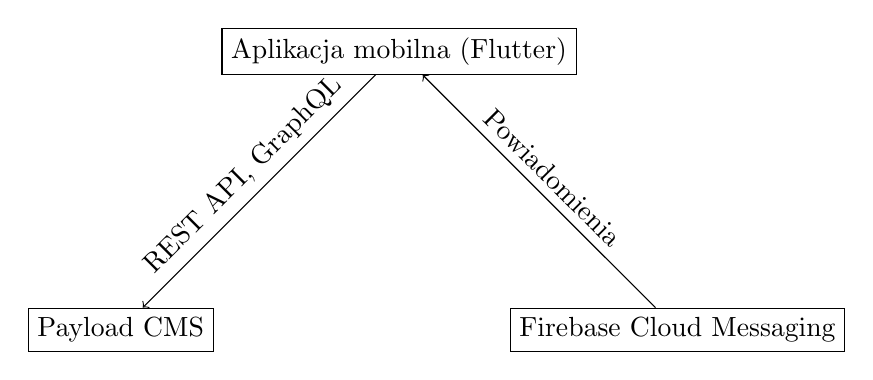
\begin{tikzpicture}[node distance=5cm]
		\node[draw,rectangle] (app) {Aplikacja mobilna (Flutter)};
		\node[draw,rectangle] (cms) [below left of=app] {Payload CMS};
		\node[draw,rectangle] (fcm) [below right of=app] {Firebase Cloud Messaging};
		\draw[->] (app) -- (cms) node[midway,above,sloped] {REST API, GraphQL};
		\draw[->] (fcm) -- (app) node[midway,above,sloped] {Powiadomienia};
	\end{tikzpicture}
	\caption{Architektura systemu}
	\label{fig:architecture}
\end{figure}
\newpage

Architektura aplikacji została zaprojektowana w modelu klient-serwer z następującymi komponentami:

\begin{itemize}
	\item \textbf{Frontend (aplikacja mobilna)}:
	      \begin{itemize}
		      \item Interfejs użytkownika w Material Design
		      \item Zarządzanie stanem aplikacji (Riverpod)
		      \item Przechowywanie danych lokalnych
		      \item Obsługa trybu offline
	      \end{itemize}

	\item \textbf{Backend (Payload CMS)}:
	      \begin{itemize}
		      \item REST API
		      \item System autoryzacji
		      \item Baza danych
		      \item Panel administracyjny
		      \item GraphQL
	      \end{itemize}

	\item \textbf{Usługi zewnętrzne}:
	      \begin{itemize}
		      \item Firebase Cloud Messaging (powiadomienia push)
	      \end{itemize}
\end{itemize}

\subsection{Framework Flutter}

Flutter to otwartoźródłowy framework opracowany przez firmę Google, służący do tworzenia wieloplatformowych aplikacji za pomocą jednej bazy kodu. Jego architektura opiera się na języku Dart, co pozwala na wydajną kompilację do kodu natywnego dla systemów Android, iOS, macOS, Windows, Linux, a także do aplikacji webowych. Główne zalety Fluttera to szybki rozwój interfejsu użytkownika, możliwość tworzenia aplikacji o wysokiej wydajności oraz wsparcie dla wzorców projektowych takich jak Material Design i Cupertino.

\subsubsection{Możliwości języka Dart}
Język Dart, na którym opiera się Flutter, jest wieloparadygmatowym językiem programowania opracowanym przez Google. Wśród jego cech charakterystycznych można wymienić:
\begin{itemize}
	\item \textbf{Statyczne typowanie}: Pozwala na wykrywanie błędów już na etapie kompilacji.
	\item \textbf{Obsługa programowania obiektowego}: Dart wspiera klasy, dziedziczenie, interfejsy i mixiny, co pozwala na tworzenie złożonych struktur kodu.
	\item \textbf{Hot Reload}: Funkcja ta umożliwia szybkie wprowadzanie zmian w kodzie i ich natychmiastowe testowanie, co przyspiesza proces rozwoju aplikacji.
	\item \textbf{Wydajność}: Kod Dart jest kompilowany do kodu natywnego, co pozwala na uzyskanie wysokiej wydajności aplikacji.
	\item \textbf{Asynchroniczność}: Obsługa asynchronicznych strumieni i przyszłości (ang. Futures) umożliwia efektywną pracę z operacjami wejścia/wyjścia.
\end{itemize}

\subsubsection{Material Design}
Flutter zapewnia natywne wsparcie dla Material Design, języka projektowania stworzonego przez Google, który definiuje zasady tworzenia nowoczesnych, responsywnych i estetycznych interfejsów użytkownika. Flutter udostępnia szeroki zestaw gotowych komponentów, takich jak:\
\begin{itemize}
	\item \texttt{AppBar} - pasek aplikacji z tytułem i opcjonalnymi akcjami.
	\item \texttt{FloatingActionButton} - unoszący się przycisk akcji.
	\item \texttt{Drawer} - wysuwane menu nawigacyjne.
	\item \texttt{Card} - komponent do wyświetlania informacji w stylu kart.
	\item \texttt{TextField} - pole tekstowe do wprowadzania danych.
\end{itemize}
Dzięki temu deweloperzy mogą tworzyć spójne interfejsy użytkownika zgodne z najnowszymi trendami projektowymi.

\subsubsection{Pakiety i narzędzie Pub}
Pub to menedżer pakietów dla Fluttera i języka Dart, który umożliwia łatwe zarządzanie bibliotekami i zależnościami w projekcie. Za pomocą Pub można:
\begin{itemize}
	\item Dodawać gotowe pakiety z \texttt{pub.dev}, takich jak \texttt{http} do pracy z protokołem HTTP czy \texttt{provider} do zarządzania stanem aplikacji.
	\item Tworzyć własne pakiety i udostępniać je społeczności programistów.
	\item Aktualizować zależności i zarządzać ich wersjami, co pozwala na utrzymanie zgodności między różnymi komponentami aplikacji.
\end{itemize}

Dzięki Pub, rozwój aplikacji w Flutterze staje się bardziej efektywny, a społeczność użytkowników ma dostęp do bogatego ekosystemu bibliotek i narzędzi.

\subsection{Payload CMS}
Payload CMS to nowoczesny system zarządzania treścią (CMS), który został zaprojektowany z myślą o deweloperach. Jest to w pełni konfigurowalny headless CMS oparty na Node.js, który umożliwia łatwe tworzenie i zarządzanie treściami w aplikacjach internetowych. Payload wyróżnia się prostotą integracji, elastycznością oraz wysoką wydajnością.

\subsubsection{Funkcje i zalety Payload CMS}
Payload CMS oferuje szereg zaawansowanych funkcji, które ułatwiają pracę deweloperom:
\begin{itemize}
	\item \textbf{Headless CMS}: Payload działa jako API-first CMS, co oznacza, że treści można dostarczać do dowolnego frontendowego frameworka lub aplikacji.
	\item \textbf{Elastyczna konfiguracja}: System pozwala na definiowanie niestandardowych schematów treści (ang. schemas) przy użyciu kodu JavaScript lub TypeScript.
	\item \textbf{Bezpieczeństwo}: Payload oferuje wbudowane mechanizmy uwierzytelniania, zarządzania użytkownikami i ról, a także obsługę protokołu OAuth.
	\item \textbf{Interfejs użytkownika}: Payload udostępnia intuicyjny panel administracyjny, który jest generowany automatycznie na podstawie zdefiniowanych schematów.
	\item \textbf{API REST i GraphQL}: Payload obsługuje zarówno REST API, jak i GraphQL, co umożliwia łatwy dostęp do danych na różne sposoby.
	\item \textbf{Wtyczki i rozszerzalność}: Payload wspiera wtyczki, co pozwala na rozszerzanie jego funkcjonalności o dodatkowe moduły.
\end{itemize}

\subsubsection{Proces tworzenia projektu}
Tworzenie projektu w Payload CMS przebiega w kilku prostych krokach:
\begin{enumerate}
	\item \textbf{Instalacja}: Payload można zainstalować za pomocą menedżera pakietów npm lub yarn:
	      \textbf{Listing. \ref{lst:cms} (s. \pageref{lst:cms})}:
	      \begin{lstlisting}[language=C++, caption=Tworznie cms , label={lst:cms}]
    npx create-payload-app my-project
    \end{lstlisting}
	\item \textbf{Definicja schematów}: Deweloperzy definiują kolekcje danych w formie kodu, np.:
	      \textbf{Listing. \ref{lst:cms2} (s. \pageref{lst:cms2})}:
	      \begin{lstlisting}[language=C++, caption=Przykład deklaracji w Payload CMS, label={lst:cms2}]
    const Posts = {
      slug: 'posts',
      fields: [
        {
          name: 'title',
          type: 'text',
        },
        {
          name: 'content',
          type: 'richText',
        },
      ],
    };
    \end{lstlisting}
	\item \textbf{Uruchomienie serwera}: Po skonfigurowaniu projektu, serwer Payload można uruchomić poleceniem \texttt{npm run dev}.
	\item \textbf{Integracja z frontendem}: Payload CMS udostępnia API, które można wykorzystać w aplikacjach frontendowych, np. z wykorzystaniem React, Next.js czy Vue.js.
\end{enumerate}

\subsubsection{Przykładowe zastosowania Payload CMS}
Payload CMS znajduje zastosowanie w wielu typach projektów, takich jak:
\begin{itemize}
	\item Strony internetowe i blogi,
	\item Aplikacje mobilne i webowe wymagające dynamicznych treści,
	\item Platformy e-commerce,
	\item Systemy zarządzania użytkownikami.
\end{itemize}

Dzięki swojej elastyczności i nowoczesnemu podejściu Payload CMS stanowi doskonałe rozwiązanie dla deweloperów poszukujących prostego w użyciu, ale jednocześnie potężnego narzędzia do zarządzania treścią.

\subsection{Projekt interfejsu użytkownika aplikacji}

\subsubsection{Style i motywy}
\begin{itemize}
	\item Spójny system projektowy Material Design 3
	\item Wsparcie dla motywu jasnego i ciemnego
	\item Dynamiczne dostosowanie do różnych rozmiarów ekranów
	\item Responsywne komponenty UI
\end{itemize}

\subsubsection{Nawigacja}
\begin{itemize}
	\item Menu dolne z 4 głównymi sekcjami:
	      \begin{itemize}
		      \item Panel główny
		      \item Powiadomienia
		      \item Wiadomości
		      \item Ustawienia
	      \end{itemize}
	\item Nawigacja stosowa między ekranami
	\item Gesty nawigacyjne (swipe)
\end{itemize}

\subsection{Model danych}

\subsubsection{Główne encje}
\begin{itemize}
	\item \textbf{User}:
	      \begin{itemize}
		      \item Dane podstawowe (imię, nazwisko, email)
		      \item Rola (student/wykładowca/admin)
		      \item Ustawienia (język, powiadomienia)
	      \end{itemize}

	\item \textbf{Schedule}:
	      \begin{itemize}
		      \item Przedmiot
		      \item Data i czas
		      \item Sala
		      \item Prowadzący
	      \end{itemize}

	\item \textbf{Notification}:
	      \begin{itemize}
		      \item Typ
		      \item Treść
		      \item Data
		      \item Odbiorcy
	      \end{itemize}
\end{itemize}

\subsection{Bezpieczeństwo}

\begin{itemize}
	\item \textbf{Autoryzacja}:
	      \begin{itemize}
		      \item JWT tokens
		      \item Refresh tokens
		      \item Szyfrowanie danych wrażliwych
	      \end{itemize}

	\item \textbf{Walidacja danych}:
	      \begin{itemize}
		      \item Walidacja formularzy
		      \item Sanityzacja danych wejściowych
		      \item Obsługa błędów
	      \end{itemize}
\end{itemize}

\subsection{Synchronizacja danych}

\begin{itemize}
	\item \textbf{Cache lokalny}:
	      \begin{itemize}
		      \item Przechowywanie planu zajęć
		      \item Buforowanie ogłoszeń
		      \item Ustawienia użytkownika
	      \end{itemize}

	\item \textbf{Strategia synchronizacji}:
	      \begin{itemize}
		      \item Automatyczna synchronizacja w tle
		      \item Ręczne odświeżanie danych
		      \item Kolejkowanie operacji offline
	      \end{itemize}
\end{itemize}
\subsection{Diagram UML}
% Klasa Student
\begin{figure}[H]
	\centering
	\begin{tikzpicture}
		\umlclass[x=0, y=0]{Student}{
			- id: int \\
			- firstName: String \\
			- middleName: dynamic \\
			- familyName: String \\
			- coursesOfStudy: List<CoursesOfStudy> \\
			- dateOfBirth: DateTime \\
			- updatedAt: DateTime \\
			- createdAt: DateTime \\
			- collection: String \\
			- loginAttempts: int
		}{
			+ factory Student.fromJson(Map<String, dynamic> json) \\
			+ toJson(): Map<String, dynamic>
		}
	\end{tikzpicture}
	\caption{Klasa Student}
	\label{fig:class-student}
\end{figure}
\newpage
% Klasa Schedule
\begin{figure}[H]
	\centering
	\begin{tikzpicture}
		\umlclass[x=0, y=0]{Schedule}{
			- id: int \\
			- courseOfStudy: int \\
			- weekAfullTimeSchedule: WeekFullTimeSchedule \\
			- weekAPartTimeSchedule: WeekPartTimeSchedule \\
			- weekBfullTimeSchedule: WeekFullTimeSchedule \\
			- weekBPartTimeSchedule: WeekPartTimeSchedule \\
			- updatedAt: DateTime \\
			- createdAt: DateTime
		}{
			+ factory Schedule.fromJson(Map<String, dynamic> json) \\
			+ toJson(): Map<String, dynamic>
		}
	\end{tikzpicture}
	\caption{Klasa Schedule}
	\label{fig:class-schedule}
\end{figure}

% Klasa CoursesOfStudy
\begin{figure}[H]
	\centering
	\begin{tikzpicture}
		\umlclass[x=0, y=0]{CoursesOfStudy}{
			- id: int \\
			- fieldOfStudy: String \\
			- faculty: Faculty \\
			- schedule: Schedule \\
			- courseType: String \\
			- levelOfStudy: String \\
			- obtainedTitle: String \\
			- numberOfSemesters: int \\
			- currentSemester: int \\
			- startDate: DateTime \\
			- endDate: DateTime \\
			- updatedAt: DateTime \\
			- createdAt: DateTime
		}{
			+ factory CoursesOfStudy.fromJson(Map<String, dynamic> json) \\
			+ toJson(): Map<String, dynamic>
		}
	\end{tikzpicture}
	\caption{Klasa CoursesOfStudy}
	\label{fig:class-coursesofstudy}
\end{figure}

\subsection{Design backendu}
Modularna i skalowalna architektura backendu stanowi kluczowy element współczesnych systemów programistycznych. Projektowanie backendu oparte na najlepszych praktykach pozwala na łatwe zarządzanie, rozwijanie oraz integrację z różnorodnymi usługami. Poniżej przedstawiono kluczowe aspekty, które powinny być uwzględnione przy projektowaniu nowoczesnego backendu.

\subsubsection{Budowa modułowa}
Budowa modułowa pozwala na podzielenie systemu na niezależne komponenty, które mogą być rozwijane i utrzymywane autonomicznie. Dzięki temu:
\begin{itemize}
	\item Każdy moduł jest odpowiedzialny za określony zestaw funkcjonalności, co ułatwia ich implementację i testowanie.
	\item Możliwe jest równoległe rozwijanie różnych części systemu przez różne zespoły deweloperskie.
	\item Moduły można łatwo wymieniać lub rozszerzać bez wpływu na pozostałe części systemu.
\end{itemize}

\subsubsection{Łatwa skalowalność}
Aby backend był skalowalny, należy:
\begin{itemize}
	\item Projektować usługi zgodnie z zasadami mikroserwisów lub serverless, co pozwala na niezależne skalowanie poszczególnych funkcjonalności.
	\item Korzystać z elastycznych baz danych, takich jak NoSQL, które łatwo adaptują się do wzrostu danych.
	\item Wykorzystać load balancery do równoważenia obciążenia między serwerami.
	\item Używać narzędzi monitorujących, takich jak Prometheus czy Grafana, aby efektywnie zarządzać wydajnością systemu.
\end{itemize}

\subsubsection{Internacjonalizacja}
Internacjonalizacja (i18n) jest kluczowa dla systemów działających na rynkach globalnych. Kluczowe kroki to:
\begin{itemize}
	\item Używanie narzędzi takich jak gettext lub formatów JSON/YAML do przechowywania tłumaczeń.
	\item Projektowanie interfejsów API, które wspierają wielojęzyczność, np. poprzez parametry \texttt{locale}.
	\item Uwzględnianie lokalnych formatów dat, liczb i walut w zależności od ustawień użytkownika.
	\item Testowanie systemu pod kątem poprawności wyświetlania treści w różnych językach.
\end{itemize}

\subsubsection{Bezpieczeństwo i zarządzanie danymi}
Bezpieczeństwo danych i użytkowników to fundament każdego backendu. Zaleca się:
\begin{itemize}
	\item Stosowanie szyfrowania danych w ruchu (TLS/SSL) oraz w spoczynku.
	\item Implementację autoryzacji i uwierzytelniania z wykorzystaniem standardów takich jak OAuth 2.0 czy JWT.
	\item Regularne testy bezpieczeństwa w celu wykrywania podatności.
	\item Spełnianie wymogów prawnych, takich jak RODO (GDPR) w przypadku zarządzania danymi osobowymi.
\end{itemize}

\subsubsection{Monitorowanie i obsługa błędów}
Monitorowanie systemu pozwala na szybkie wykrywanie i rozwiązywanie problemów. Warto:
\begin{itemize}
	\item Korzystać z narzędzi takich jak Sentry do logowania błędów.
	\item Implementować mechanizmy automatycznego restartu usług w przypadku awarii.
	\item Tworzyć raporty wydajnościowe i systemy alertów w celu bieżącej kontroli stanu backendu.
\end{itemize}

Modularna budowa, łatwa skalowalność, internacjonalizacja, bezpieczeństwo oraz monitorowanie stanowią podstawę dobrze zaprojektowanego backendu, który może sprostać wymaganiom współczesnych aplikacji.
